\section{The Dataset}

For purposes of the project, we have chosen to use the Microsoft Common Objects in Context, a dataset of over 330 thousand images, with over 200 of these labeled, 80 categories of instances, and over 1.5 million object instances all together (\citeA{COCOdataset}). This substantial dataset is utilized with an API developed specifically to access the contents of the dataset, both of which have been made open-source by their developers \href{https://github.com/cocodataset/cocoapi}{(Link to the API)}. The objectives of MSCOCO are to detect and categorize objects found within images based on their iconicity, their position in relation to other objects, and the binding coordinates of space they occupy in a given image. 


\subsection{Properties of Data}
Notably, MSCOCO is proposed by its developers to be more effective at training object recognition models than other popular datasets that are used in research and the industry. These advantages of MSCOCO mainly lay in the following properties of the data and the dateset.


\begin{enumerate}
    \item Detecting non-iconic views \begin{itemize}
        \item In line with its focus of detecting images in their natural contexts, MSCOCO is designed to be more effective in detecting objects in non-iconic views than other datasets. When speaking to what iconicity means in this context, we mean a recognition system’s ability to interpret objects from an image, even when those objects are obscured by clutter, and layered deep behind occlusions which move them away from the image’s center-focus.
        \item On average, MSCOCO’s objects are smaller when compared to the sizes found in other popular datasets such as ImageNet and PASCAL, a feature which speaks to its greater efficiency at parsing through ambiguity and noise to detect the intended objects.
        \end{itemize}
    \item Contextual Reasoning
        \begin{itemize}
            \item MSCOCO also uses contextual reasoning where multiple objects are present, which demonstrates the improved ability to recognize them even when objects are not isolated, and are instead present amongst others. For instance, where previous datasets, such as ImageNet and PASCAL, account for 60\% of their images being object-isolated (meaning only depict a singular object), MSCOCO account for only 10\%. The processing of such contextually-ambiguous scenes further builds onto the dataset’s ability to object-recognize in natural scenes, and not just scenes where the object of interest is centrally-focused. 
        \end{itemize} 
    \item Object localization
        \begin{itemize}
            \item Given the effort MSCOCO places on contextual reasoning, and the importance of parsing through non-iconic scenes, it’s important to also understand that (a) MSCOCO requires, and indeed has, the ability of object localization–that is, the ability to process the spatial relations between objects in a scene; and (b), how MSCOCO segments this object localization.
        \end{itemize}
\end{enumerate}

\subsection{Functionality of Data}

When observed, the dataset can first be categorized by the type of objects being analyzed, and secondly by what object of the category is being analyzed. 

Of the 80 categories offered, we focus on 10, which can be classified as animals: bird, cat, dog, horse, sheep, cow, elephant, bear, zebra, and giraffe. Using this dataset, we aim to train a spiking neural network to demonstrate the intended object-recognition model.

Functionally, when an image is analyzed, the program identifies key attributes which are used to categorize appropriately. For instance, where we analyze an image of two giraffes, we should consider the properties of the data used in the process of segmentation.

\begin{figure}[h]
	\begin{center}
		\scalebox{0.4}{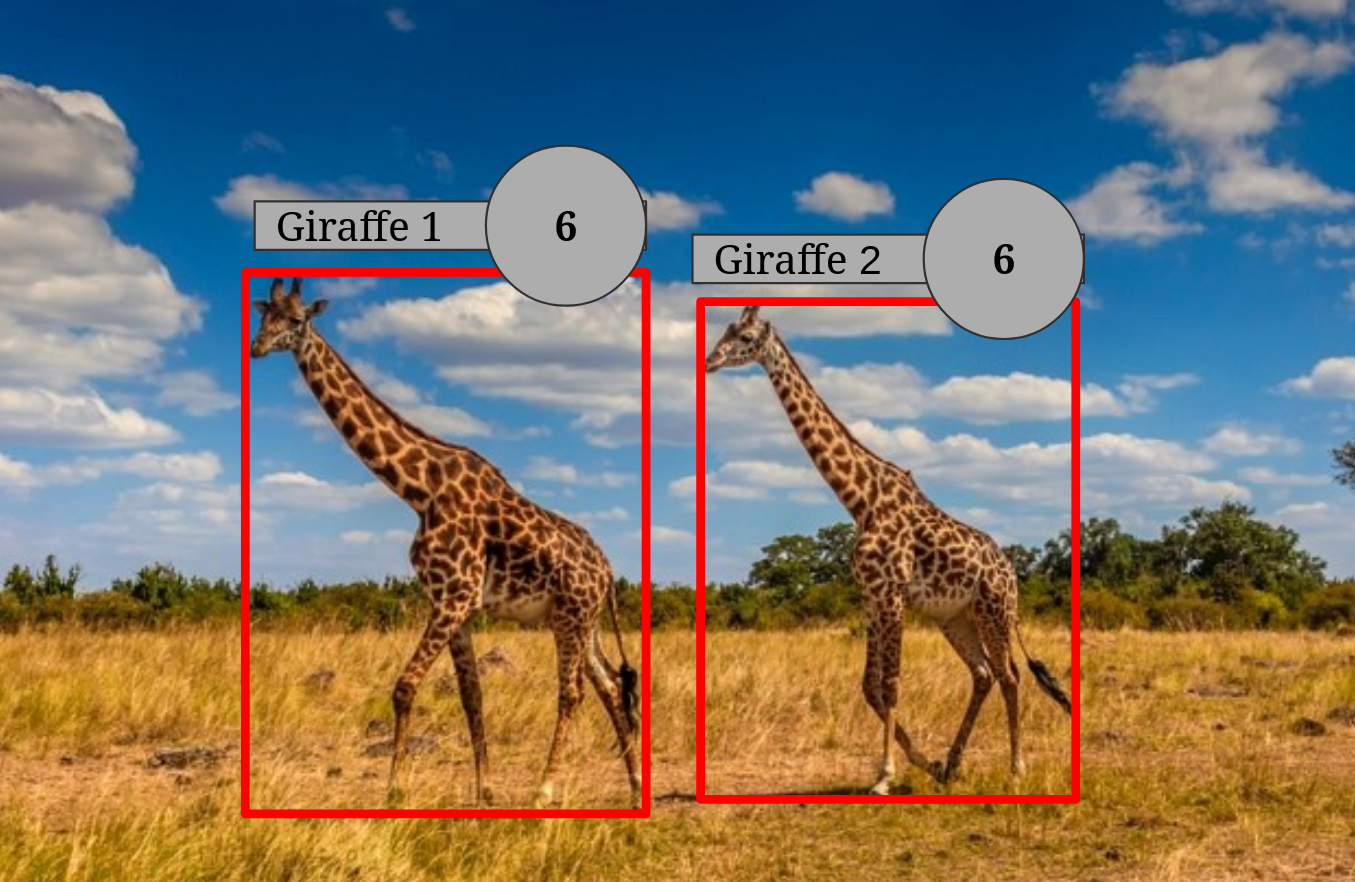
\includegraphics{giraffe.png}}
	
	\end{center}
	\caption{Example of an image from the MSCOCO dataset with the annotations that it contains.}
\end{figure}

\begin{enumerate}
    \item Boxes 
        \begin{itemize}
        \item The image presented is first identified by a “bounding box”; this box is important for object localization. It provides the minimum and maximum coordinates along a cartesian-plane to identify the boundaries of space an object occupies.
        \end{itemize}
    \item Area
        \begin{itemize}
            \item Within the bounding box, a pixel count for each object present is processed and utilized to further understand the iconicity and/or ambiguity of the object in relation to its scene.
        \end{itemize} 
    \item Label
        \begin{itemize}
            \item This property output can be read to distinguish (a) the number of object-instances found in an image, and (b) the category each object-instance.
        \end{itemize}
\end{enumerate}


\begin{wrapfigure}[25]{r}{0.42\textwidth}
	\begin{center}
		\scalebox{0.45}{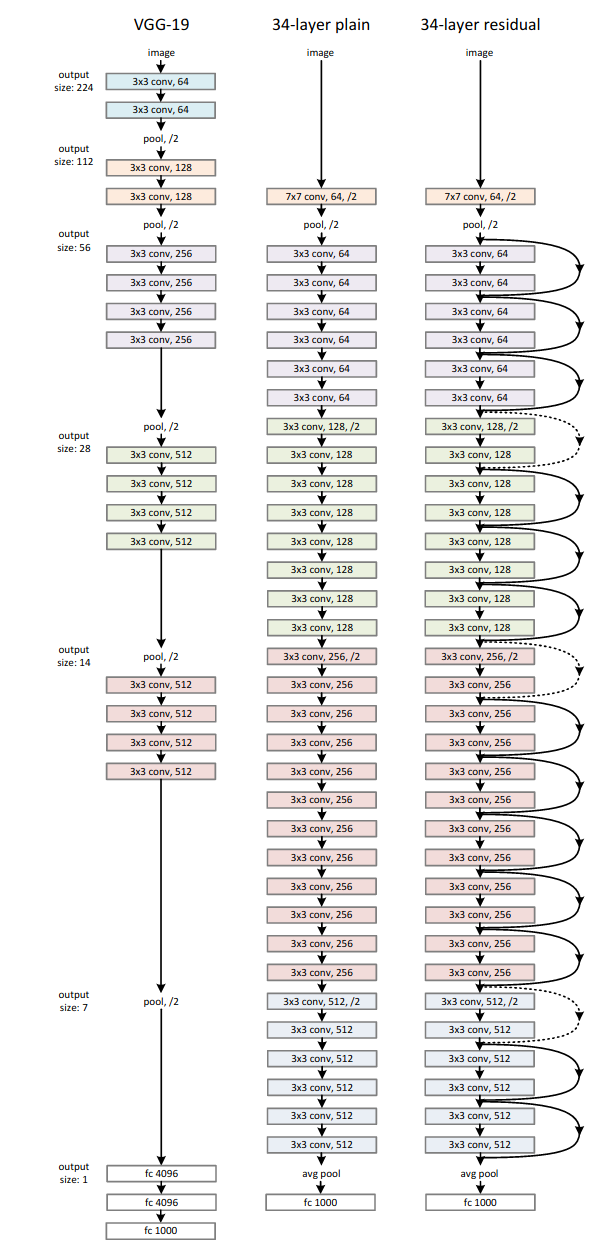
\includegraphics{resnet_comp.png}}
	\end{center}
		\caption{Examples of 16-layer VGG, Plain 34-layer, and 34-layer ResNet Network 
		Architectures}
\end{wrapfigure}

The described properties of the image annotation should be considered in relation to the process segmentation in object recognition. Mainly, it’s important to consider that object-segmentation is a difficult process and requires an accurate bounding boxes prediction. Furthermore, considering that the dataset holds over 1.5 million category instances, given the sheer magnitude and complexity of the dataset efficiency plays a big role in training a neural-network that utilizes this dataset. As such, a major goal of our assignment is to build and train a spiking neural network model to do so.  
